\documentclass[12pt,a4paper]{article}
\usepackage{amsmath}
\usepackage{mathtext}
\usepackage{icomma}
\usepackage{amsfonts}
\usepackage{amssymb}
\usepackage[utf8]{inputenc}
\usepackage[T1,T2A]{fontenc}
\usepackage[english, russian]{babel}
\usepackage{graphicx}
\usepackage[left=2cm,right=2cm,top=2cm,bottom=2cm]{geometry}
\usepackage{calc}
\usepackage{wrapfig}
\usepackage{setspace}
\usepackage{indentfirst}
\usepackage{subfigure}
\usepackage[table,xcdraw]{xcolor}
\usepackage{float}

\title{Отчет о выполнении лабораторной работы 3.4.2\\
Закон Кюри-Вейсса}

\author{Исламов Сардор, группа Б02-111}
\date{26 ноября 2022 г.}

\begin{document}
\maketitle
\subparagraph*{Аннотация.} 
В работе исследована зависимость периода колебаний автогенератора от температуры сердечника катушки.
По результатам измерений определена парамагнитная точка Кюри гадолиния.

\subsection*{Теоретическое введение}
Вещества с отличными от нуля атомными магнитными моментами обладают парамагнитными свойствами. 
Внешнее магнитное поле ориентирует магнитные моменты, которые в отсутствие поля располагались в пространстве хаотическим образом. 
Однако при $T \rightarrow 0$ тепловое движение всё меньше препятствует магнитным моментам атомов ориентироваться в одном направлении при сколь угодно слабом внешнем поле. 
В ферромагнетиках -- под влиянием обменных сил -- это происходит при понижении температуры не до абсолютного нуля, а до температуры Кюри $\Theta$. 
Оказывается, что у ферромагнетиков магнитная восприимчивость должна удовлетворять закону Кюри-Вейсса:
\begin{equation}
    \label{eq:Kuri-Veicca}
    \chi \propto \frac{1}{T-\Theta_p},
\end{equation}
где $\Theta_p$ -- температура, близкая к температуре Кюри, так как при $T \approx \Theta$ формула~(\ref{eq:Kuri-Veicca}) недостаточна точна.

\subsection*{Экспериментальная установка}
Схема установки для проверки закона Кюри-Вейсса показана на рис.~\ref{ris:ustanovka}. Исследуемый ферромагнитный образец (гадолиний) расположен внутри пустотелой катушки самоиндукции, которая служит индуктивностью колебательного контура, входящего в состав LC-автогенератора. 
Автогенератор собран на полевом транзисторе КП-103 и смонитрован в виде отдельного блока.
\begin{figure}[H]
    \centering
    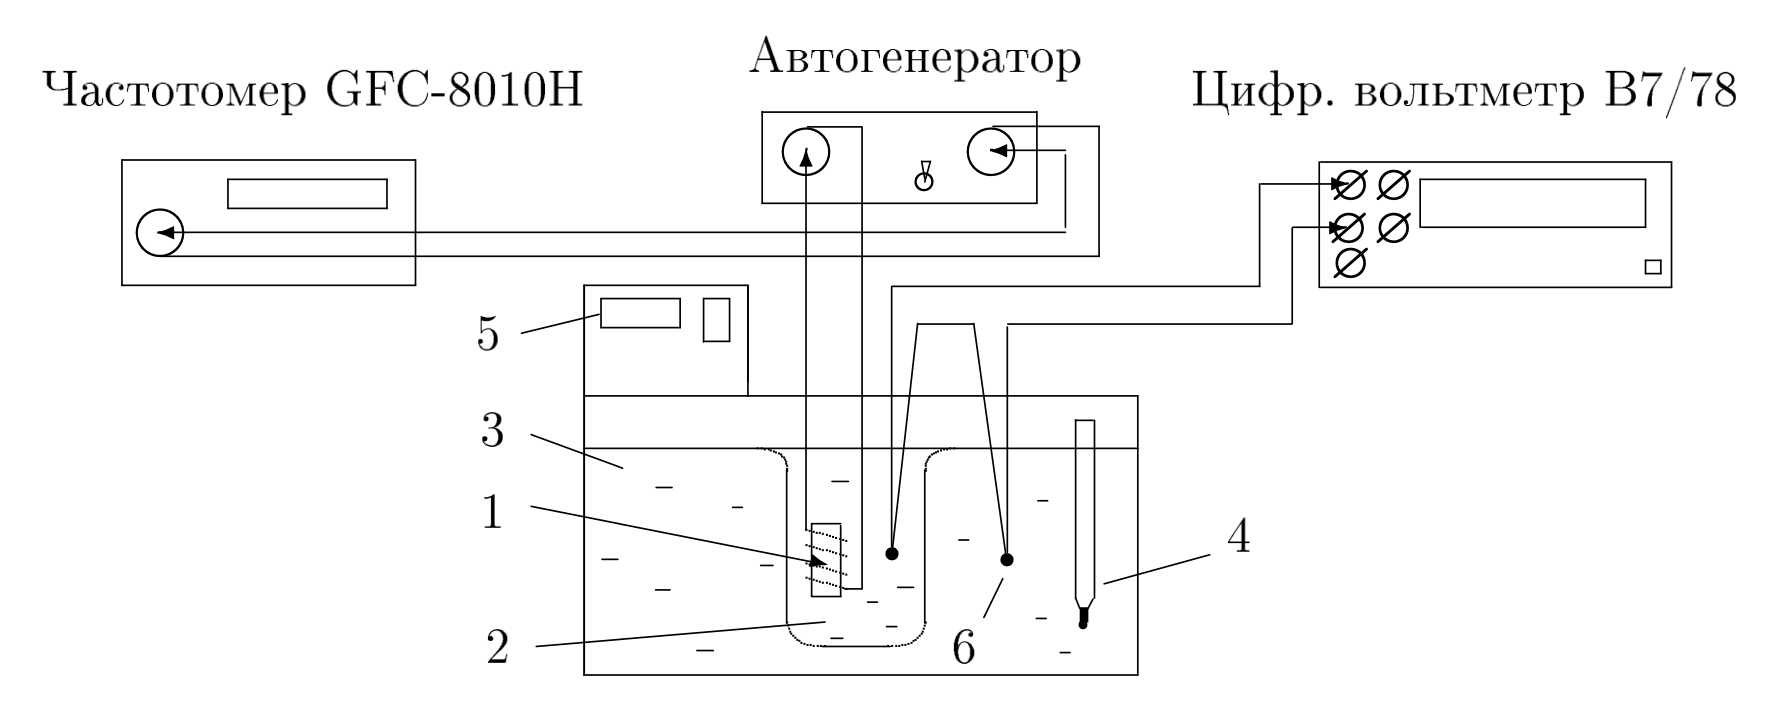
\includegraphics[width=0.7\linewidth]{pics/scheme.png}
    \caption{Схема экспериментальной установки.}
    \label{ris:ustanovka}
\end{figure}

Магнитная воосприимчивость образца $\chi$ определяется по изменению самоиндукции катушки. 
Обозначив через $L$ самоиндукцию катушки с образцом и через $L_0$ -- её самоиндукцию в отсутствие образца, получим
\[
    (L-L_0)\propto \chi.
\]

При изменении самоиндукции образца меняется период колебаний автогенератора:
\[    \tau = 2\pi \sqrt{LC}, \]
где $C$ -- ёмкость конутра автогенератора. Период колебаний в отсуствие образца опредлеяется самоиндукцией пустой катушки:
\[    \tau_0 = 2\pi \sqrt{L_0C}. \]

Итак, закон Кюри-Вейсса справедлив, если выполнено соотношение:
\begin{equation}
    \frac{1}{\chi} \propto (T-\Theta_p) \propto \frac{1}{\tau^2-\tau_0^2}
\end{equation}

\subsection*{Результаты измерений и обработка данных}

\subsection*{Подведение итогов}
\end{document}